\documentclass[]{scrartcl}
\title{Vorlesung Analysis II}
\usepackage{amsmath,amssymb,amsfonts}
\usepackage{stmaryrd}
\usepackage{mathtools}
\usepackage{latexsym}
\usepackage{graphicx}
\usepackage{tikz}
\usepackage{xcolor}
\usepackage[most]{tcolorbox}
\usepackage{soul}
\usepackage{ upgreek }
\usepackage{hyperref}
\usepackage{tipa}
\usepackage[dvipsnames]{xcolor}
\hypersetup{
	colorlinks=true,
	linkcolor=blue,
	filecolor=magenta,      
	urlcolor=cyan,
	pdftitle={Overleaf Example},
	pdfpagemode=FullScreen,
}
\newcommand{\redcircle}[1]{%
	\tikz[baseline=(char.base)]{
		\node[shape=circle, draw=red, text=red, thick, inner sep=1pt] (char) 
		{\textbf{#1}};
	}%
}
\newcommand{\bluecircle}[1]{%
	\tikz[baseline=(char.base)]{
		\node[shape=circle, draw=blue, text=blue, thick, inner sep=1pt] (char) 
		{\textbf{#1}};
	}%
}
\newcommand{\blackcircle}[1]{%
	\tikz[baseline=(char.base)]{
		\node[shape=circle, draw=black, text=black, thick, inner sep=1pt] 
		(char) 
		{\textbf{#1}};
	}%
}
\newcommand{\orangecircle}[1]{%
	\tikz[baseline=(char.base)]{
		\node[shape=circle, draw=orange, text=orange, thick, inner sep=1pt] 
		(char) 
		{\textbf{#1}};
	}%
}
\newcommand{\redul}[1]{\setulcolor{red}{\ul{#1}}}
\newcommand{\blueul}[1]{\setulcolor{blue}{\ul{#1}}}
\newcommand{\yelul}[1]{\setulcolor{yellow}{\ul{#1}}}
\newcommand{\greenul}[1]{\setulcolor{green}{\ul{#1}}}
\newcommand{\oraul}[1]{\setulcolor{orange}{\ul{#1}}}
\setul{1pt}{3pt} % Linienhöhe und Abstand zum Text (optional anpassbar)

\setlength{\topmargin}{-.5in} \setlength{\textheight}{9.25in}
\setlength{\oddsidemargin}{0in} \setlength{\textwidth}{6.8in}
\setlength{\parindent}{0pt}

\begin{document}
	\maketitle
	\textbf{\underline{Teil 1: Differentialrechnung im $\mathbb{R}^n$}}\\
	\\
	\textbf{\underline{an9: Extrema mit Nebenbedingungen, implizierte 
	Funktionen}}\\
	\\
	\textbf{\underline{\underline{Stichworte:}Extrma mit NBen, 
	Lagrange-Multiplikationen, implizierter Funktionensatz}}\\
	\\
	\textbf{\underline{Literatur}} \blueul{[Hoff], Kapitel 9.8, [Forster], 
	Kapitel 8,9}\\
	\\
	\textbf{9.1. \underline{Einleitung:}} Sla Anwendung des Satzes von der 
	lokalen Umkehrbarkeit zeigen wir den impliziten Funktionensatz und 
	untersuchen Extrema mit Nebenbedingungen.\\
	\\
	\textbf{9.2 \underline{Motivation:}} Sei $a \in U\subset \mathbb{R}^n, 
	f:U\rightarrow \mathbb{R}$. Diskutieren im Fall \underline{n=2:}\\
	\underline{1. Ziel:} Wollen die Glg. f(x,y)=0 "nach y auflösen", also eine 
	Fkt. l finden mit \greenul{$f(x,y)=0\Leftrightarrow y=l(x)$}. Wir sagen 
	dann, die Glg. f(x,y)=0 definiert \underline{implizit} eine FUnktion l. Wie 
	und unter welcher Vor. das geht, beschreibt der Satz über implizite 
	Funktionen. Wir erwarten, das dies nur "lokal" geht, also auf Umgebungen 
	einer Stelle a und einem Wert b mit f(a,b)=0.
	\begin{figure}[h]
		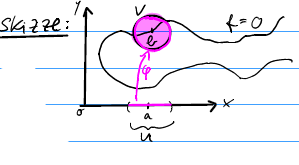
\includegraphics[width=5 cm,height=3cm]{bsp kap 9.2}
	\end{figure}\\
	\underline{Konkretes Bsp.:} Glg. $x^2+4y^2=1 \rightarrow 
	f(x,y)=x^2+4y^2-1$, und $y= \pm \frac{1}{2}\sqrt{1-x^2}.$\\
	\underline{2. Ziel:} Bsp. \underline{n=2}\\
	In Anwendungen er Extremwertbestimmung wird oft nach Extrema von Funktionen 
	g(x,y) auf einer \redul{Nullstellenmenge}\yelul{N}$:=\{(x,y)\in \mathbb^2; 
	f(x,y)=0\}$ gefragt, d.h. \greenul{unter der Bedingung f(x,y)=0}. Gegeben 
	ist dann eine \redul{"Nebenbedingung"}.\\
	\underline{Konkretes Bsp.:} $\overline{f}(x,y)=\frac{xy}{1+x^4+y^4}$, ist 
	stetig, nimmt Extrema auf $N=\{(x,y);f(x,y)=0\}$ an. Ist $\begin{pmatrix}
		x_0\\y_0
	\end{pmatrix}\in N$ so eine Stelle, und ist $\begin{pmatrix}
		-1\\0
	\end{pmatrix}\neq\begin{pmatrix}
		x_0\\y_0
\end{pmatrix}\neq\begin{pmatrix}
		1\\0
\end{pmatrix}$, dann gilt nahe $\begin{pmatrix}
		x_0\\y_0
\end{pmatrix}: D_2f(x,y)\neq 0$.\\
	\begin{figure}[h]
		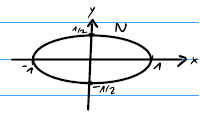
\includegraphics[width=5 cm,height=3cm]{bsp kap 9.2.2}
	\end{figure}\\
	\\
	\textbf{9.3. \underline{Allgemeine Situation:}} Sei $D\subset \mathbb{R}^n, 
	2\leq l \leq n, (f_1,...,f_l)=f\in l^1(D,\mathbb{R}^l)$.\\
	Setze \redul{$N:=\bigcap_{1=2}^l f^{-1}_i(0)$}, ist offen in 
	$\mathbb{R}^n$,\\
	Sprechweise: $f_1$ hat ein \redul{lokales Etremum in $a\in N$} mit 
	\redul{Nebenbedingung N}, falls $f_{1/N}$ in a ein lokales Extremum hat.\\
	\\
	\textbf{9.4. \underline{Satz:}} Geg. die \blueul{Situation 9.3}, 
	\underline{Vor.:} $f_{1/N}$ hat \greenul{in $a\in N$ ein lokales 
	Extremum}.\\
	\underline{Beh.:} rg $\begin{pmatrix}
		D_1f_1&\cdots&D_nf_1\\
		\vdots&&\vdots\\
		D_1f_l&\cdots&D_nf_l
	\end{pmatrix}(a) \textless l.$ \redul{"Lagrangesche Multiplikatorenregel"}\\
	\\
	\textbf{9.5. \underline{Bem.:}} $\bullet$ Im Fall l=n ist die Beh. 
	äquivalent zu $\begin{pmatrix}
		D_1f_1&\cdots&D_nf_1\\
		\vdots&&\vdots\\
		D_1f_n&\cdots&D_nf_n
	\end{pmatrix}(a)=0.$\\
	$\bullet$ Es gilt: Beh. $rg(...)\textless l$\\
	$\Leftrightarrow f_1'(a),...,f_l'(a)$ sind Lin. abh.\\
	$\Leftrightarrow \in (\overline{\lambda_1},...,\lambda_l)^T 
	\in\mathbb{R}^l\backslash\{0\}. 
	D_j(\sum_{i=1}^{l}\overline{\lambda_i}f_i)(a)=0$ für alle 
	$j\in\{1,...,n\}$.\\
	\OE sei $\lambda_1=1$(sonst unnumerieren und normieren).\\
	Also $\exists(\lambda_2,...,\lambda_l)^T\in\mathbb{R}^{l-1}$ mit 
	$D_jf_1(a)=\sum_{i=2}^{l}\lambda_iD_jf_i(a),$ alle $j\in\{1,...,n\}$.\\
	$\Rightarrow f_1(a)=\sum_{i=2}^{l}$\yelul{$\lambda_i grad 
	f_i(a)$}.\textopencorner \OE Ohne Minus vor den $\lambda_i$...\textcorner\\
	\textopencorner Bsp. für $l=2: \exists \lambda\in\mathbb{R}:grad 
	f_1(a)=\lambda grad f_2(a),$ für $f_2'(a)\neq 0$.\textcorner\\
	\\
	\textbf{9.6. \underline{Def.:}} Man nennt die $\lambda_2,...,\lambda_l$ 
	\redul{Lagrargemultiplikatoren}.\\
	\\
	\textbf{9.7. \underline{Bew.:}} Sei $\OE a = 0$. $\bullet$ Ferner betr. 
	zunächst den Fall \underline{l=n}.\\
	\underline{Angenommen}, es wäre sonst \oraul{rg A=n}, wo $\begin{pmatrix}
		D_1f_1&\cdots&D_nf_1\\
		\vdots&&\vdots\\
		D_1f_n&\cdots&D_nf_n
	\end{pmatrix}(0)\in\mathbb{R}^{nxm}.$\\
Dann ist \oraul{A eine invertierbare Matrix.}\\
	Der \blueul{Satz über lokale Umkehrbarkeit 8.8} liefert dann:\\
	$\exists U \subset \mathbb{R}^n \exists V \subset \mathbb{R}^n, o \in U, 
	f(o)\in V, U\xrightarrow{fru} V$ invertierbar und bijektiv.
	
	
	
	
	
	
	
	
	
	
	
	\textbf{9.13\setulcolor{red}\ul{Satz über implizite Funktionen:}} $l,k \in \mathbb{R}^{j+k}, f\in l^1(D,\mathbb{R}^k)$\\
	\underline{Vor.:} $w\in D,F(w)=0, det(\frac{\delta f}{\delta y}(w))\neq 0 (w=(a,b)\in\mathbb{R}^lx\mathbb{R}^k).\\$
	\underline{Beh.:} $\exists U,V$ \setulcolor{green} \ul{$w\in U x V c \mathbb{R}^lx\mathbb{R}^k$} mit: \\
	\ul{$l:U\rightarrow V, x\rightarrow y \in V$ mit f(x,y)=0 ist eine Abbildung} und zwar 
	\ul{$l \in l^1 (U,\mathbb{R}^k)$.}\\
	Die Abbildung von l ist \ul{$l'(x)=*-(\frac{\delta f}{\delta y}\begin{pmatrix}x\\l(x)
		\end{pmatrix})^{-1}\frac{\delta f}{\delta x}\begin{pmatrix}
		x\\l(x)
	\end{pmatrix}$} $\in \mathbb{R}^{kxl}$.\\
	1.\underline{Bem.:} \ul{$f\in l^r$} $\xRightarrow{vollst. Ind}$ \ul{$l\in l^r$}.\\
	2.\underline{Bem.:} Bemerkenswert ist an diesem Satz, dass u.U. l nur schwierig berechnet werden kann, sehr wohl aber die Ableitung l'(x) nach der Formel (ohne die explizite Fkt. l ableiten zu müssen).\\
	\\
	\textbf{9.14.\underline{Bew.:}} $\bullet$ \underline{Falls} l existiert und diffbar, so gilt:\\
	\begin{equation}
		0=f(x,l(x))\Rightarrow (f(x,l(x)))'= 0\\
		\xRightarrow[]{K.R} \frac{\delta}{\delta x} f(x, l(x)) \cdot \frac{\delta x}{\delta x}+ \underbrace{\frac{\delta}{\delta y} f(x,l(x))}\cdot l'(x)=0\\
		\text{invbar, falls x nahe a, d.h. falls (x, l(x)) nahe (a,b)=w:}\\
		det\frac{\delta f}{\delta y}(w)\neq 0\Rightarrow det \frac{\delta f}{\delta y}(x,l(x))\neq 0\\
		\Rightarrow l'(x)=-(\frac{\delta f}{\delta y}(x, l(x))){-1} \frac{\delta f}{\delta x}(x, l(x))\Rightarrow l \in l^1.
	\end{equation} 
	$\bullet$\underline{Betr.}\begin{equation}
		F: D \rightarrow \mathbb{R}^lx\mathbb{R}^k, F\in l^1, (x,y)\rightarrowtail (x,f(x,y)).\\
		\text{Es gilt} F'(x,y)= \begin{pmatrix}
			I_l & 0\\
			\delta f & \delta f\\
			\delta x & \delta y
		\end{pmatrix} \in \mathbb{R}^{(l+k)x(l+k)}, det F' = det \frac{\delta f}{\delta y}\neq 0 \text{nahe w}.
	\end{equation}
	Der \setulcolor{blue}\ul{Satz üver lokale Umkehrbarkeit 8.8} liefert nun:\\
	$\exists W,w \in W c  \mathbb{R}^lx\mathbb{R}^k:$\\
	\begin{equation}
		\stackrel{\mathbb{R}^lx\mathbb{R}^k}{(x,y)}
	\end{equation}
	
	
\end{document}